%Η θερμική ατμόσφαιρα του ορίζοντα μιας μη φορτισμένης μελανής %οπής, αποτέλεσμα κβαντικών διακυμάνσεων του κενού, μεταφέρεται %στο άπειρο υπό τη μορφή ακτινοβολίας Hawking. 
Στην παρουσία ισχυρού μαγνητικού πεδίου, πέραν της ακτινοβολίας Hawking, αναμένεται να εκδηλωθούν φαινόμενα όπως η δίδυμος γένεση φερμιονίων-αντιφερμιονίων. Επομένως, χρειάζεται να μελετήσουμε φερμιονικά πεδία στην παρουσία πεδίου μαγνητικού μονοπόλου. Θα μελετήσουμε πρώτα το μη σχετικιστικό πρόβλημα, ενός φορτισμένου σωματιδίου στην παρουσία ενός τέτοιου μαγνητικού πεδίου, ακολουθώντας την εργασία του Haldane \cite{PhysRevLett.51.605}. 
%ο Haldane αναπτύσσει τις μη-σχετικιστικές, μονοσωματιδιακές %συναρτήσεις εντοπισμένες σε σφαιρική επιφάνεια ομόκεντρη με %μαγνητικό μονόπολο και καταλήγει στην κβάντωση του συστήματος %στα επίπεδα Landau, κάθε ένα από τα οποία αντιστοιχεί σε μια %ιδιοτιμή της ενέργειας.

\section{Σφαιρικές λύσεις στην απουσία μαγνητικού μονοπόλου}
Η χαμιλτονιανή ελέυθερου, μη σχετικιστικού σωματιδίου είναι 
\begin{equation}
    H \,=\, \frac{\Vec{p}\superscr{\,2}}{2m}
\end{equation}
με τον τελεστή της ορμής να δίδεται από τη σχέση 
\begin{equation*}
\begin{split}
    &\Vec{p}\,\equiv\,-i\hbar\vec{\nabla}\\
    &\left[ H, \Vec{p} \right]\,=\,0
\end{split}
\end{equation*}
Οι στάσιμες, χωριζόμενες λύσεις της εξίσωσης Schrödinger είναι 
\begin{equation}
    \psi\text{\scalebox{0.7}{($r,\,t$)}}\sim e\superscr{\frac{i}{\hbar}(p\cdot r - Et)}
\end{equation}
όπου $p$ το μέτρο της ορμής και $E=\frac{p^2}{2m}$ η τιμή της ενέργειας (ή η αντίστοιχη ιδιοτιμή της χαμιλτονιανής).\\

Θα επιβάλουμε τώρα, το σωματίδιο να κινείται στην επιφάνεια μιας σφαίρας. Η χαμιλτονιανή μπορεί να γραφεί 
%στην πιο βοηθητική μορφή, 
συναρτήσει της στροφορμής, η οποία διατηρείται σταθερή 
\begin{equation}\label{angular momentum operator}
    \Lambda\superscr{i} \,=\, \epsilon\superscr{ijk}r\superscr{j}p\superscr{k}
\end{equation}
Χρησιμοποιώντας την ταυτότητα $\epsilon\superscr{ijk}\epsilon\superscr{mnk}=\de\superscr{im}\de\superscr{jn}-\de\superscr{in}\de\superscr{jm}$ και τον μεταθέτη $[r\superscr{i},p\superscr{j}]\,=\,i\hbar\de\superscr{ij}$ βρίσκουμε τη στροφορμή στο τετράγωνο
\begin{equation*}
    \Vec{\Lambda}\superscr{2}\,=\,r\superscr{2}p\superscr{2}+i\hbar\,\Vec{r}\cdot\Vec{p}-(\Vec{r}\cdot\Vec{p})\superscr{2}
\end{equation*}
Σημειώνουμε ότι το διάνυσμα θέσης είναι πάντα κάθετο στην ορμή (κίνηση κατά μήκος σφαιρικής επιφάνειας) και έτσι καταλήγουμε  στη σχέση
\begin{equation}
    \Vec{r}\cdot\Vec{p}\,=\,0\,\,\Rightarrow\,\, p\superscr{2}=\frac{\Lambda\superscr{2}}{r\superscr{2}}
\end{equation}
Συνεπώς, η χαμιλτονιανή γράφεται
\begin{equation}
    H\,=\,\frac{|\Lambda|\superscr{2}}{2mr\superscr{2}}
\end{equation}
Επειδή ο μεταθέτης
\begin{equation*}
    \left[ H,\,\Vec{\Lambda} \right] \,=\, 0
\end{equation*}
μηδενίζεται, η στροφορμή $\Vec{\Lambda}$ διατηρείται. Οι συνιστώσες της στροφορμής \eqref{angular momentum operator} ικανοποιούν την $SU(2)$ άλγεβρα των περιστροφών 
\begin{equation}
    [\Lambda\superscr{i},\Lambda\superscr{j}]\,=\,i\epsilon\superscr{ijk}\Lambda\superscr{k}
\end{equation}
Η στροφορμή στο τετράγωνο είναι κβαντισμένη με ιδιοτιμές
\begin{equation}\label{eigenvalues of L squared}
    |\Vec{\Lambda}|^2\,=\,\hbar^2\,\ell(\ell+1)\quad\,\,\ell=0,1,2,\dots
\end{equation}
Οι αντίστοιχες ιδιοσυναρτήσεις  
%\eqref{eigenvalues of L squared}, την ορθοκανονική βάση των
είναι οι σφαιρικές αρμονικές
\begin{equation}
\begin{split}
    &\Lambda\superscr{2}\,\,Y\superscr{m}\subscr{\ell}\text{\scalebox{0.7}{$(\theta,\phi)$}}\,=\,\hbar\ell(\ell+1)\,\,Y\superscr{m}\subscr{\ell}\qquad \ell\,=\,0,1,2,\dots\\
    &\Lambda\subscr{z}\,\,Y\subscr{\ell}\superscr{m}\text{\scalebox{0.7}{$(\theta,\phi)$}}\,=\,\hbar m\,\,Y\subscr{\ell}\superscr{m}\qquad -\ell\le m \le\ell
\end{split}
\end{equation}
οι οποίες απαρτίζουν μια πλήρη ορθοκανονική βάση. Με βάση τις σφαιρικές αρμονικές βρίσκουμε τις στάσιμες, χωριζόμενες λύσεις της εξίσωσης Schrodinger.
Η κατάσταση ελάχιστης ενέργειας 
%προκύπτει για $\ell = 0$ με τη 
είναι η σφαιρικά συμμετρική αρμονική $Y\superscr{o}\subscr{o}=\frac{1}{2}\frac{1}{\sqrt{\pi}}$. 
%Ο γενικός εκφυλισμός των ιδιοτιμών εξαφανίζεται στη %συγκεκριμένη περίπτωση, μια σημαντική διαφορά με την περίπτωση %του κεντρικού μαγνητικού πεδίου που εξετάζεται στην επόμενη %ενότητα.

\section{Σφαιρικές λύσεις στην παρουσία μαγνητικού μονοπόλου}
Το πεδίο του μαγνητικού μονοπόλου δίδεται από τη σχέση
%καθορίζεται από την \eqref{centralB} σε συνδυασμό με την %κβάντωση Dirac $q\subscr{m}\,=\,\frac{\hbar}{2e}$ (c=1)
\begin{equation}\label{radial magnetic field}
    \Vec{B}\,=\,\frac{\hbar s\subscr{0}}{e r^2}\,\hat{\Omega} \qquad\,\,\hat{\Omega}\,=\,\frac{\Vec{r}}{r}
\end{equation}
όπου $2s\subscr{0}$ ο λόγος της συνολικής μαγνητικής ροής προς τη στοιχειώδη μαγνητική ροή $\Phi_0$
\begin{equation}
    \frac{\Phi}{\Phi\subscr{0}}\,=\,2 s\subscr{0} \qquad s\subscr{o}=1,2,\dots
\end{equation}
Η στοιχειώδης μαγνητική ροή ισούται με
\begin{equation}
    \Phi\subscr{0}\,=\,4\pi R^2B\subscr{0}\,=\,\frac{2\pi\hbar}{e}
\end{equation}
Η χαμιλτονιανή ενός μη σχετικιστικού ηλεκτρονίου, με αρνητικό φορτίο $-e$, το οποίο αλληλεπιδρά με διανυσματικό δυναμικό $\vec{A}$, η στροφή του οποίου παράγει το μαγνητικό πεδίο 
\begin{equation*}
    \epsilon\superscr{ijk}\nabla\superscr{j}A\superscr{k}\,=\,|\Vec{B}|\,\Omega\superscr{i}\qquad i,j,k=\{x,\y,z\}
\end{equation*}
ισούται με
\begin{equation*}
    H\,=\,\frac{1}{2m}\left( \Vec{p} + e\Vec{A} \right)^2 
\end{equation*}
%όπου $\Vec{p} = -i\hbar\nabla$ ο γεννήτορας μεταθέσεων και
Ο τελεστής $\Vec{\text{Π}}\equiv\Vec{p}+e\Vec{A}$ είναι η μηχανική ορμή του ηλεκτρονίου \cite{Sakurai:1167961}. Γενικά για ένα σωματίδιο με αρνητικό φορτίο $-q$, οι συνιστώσες του τελεστή της μηχανικής ορμής ικανοποιούν τις ακόλουθες σχέσεις μετάθεσης
\begin{equation}\label{mechanical momentum commutator}
\begin{split}
    [\Pi\superscr{i},\Pi\superscr{j}]&=\,[p\superscr{i},qA\superscr{i}]+[qA\superscr{i},p\superscr{j}]\,=\,-qi\hbar \nabla\superscr{i}A\superscr{j}+qi\hbar\nabla\superscr{j}A\superscr{i}=\\
    &=\,i\hbar q\left(-\de\superscr{im}\de\superscr{jn}+\de\superscr{jm}\de\superscr{in}\right)\nabla\superscr{m}A\superscr{n}\,=\,-i\hbar q \epsilon\superscr{ijk}\epsilon\superscr{mnk}\nabla\superscr{m}A\superscr{n}=\\
    &=\,-i\hbar q \epsilon\superscr{ijk}B\superscr{k}
\end{split}
\end{equation}
Η στροφορμή στην \eqref{angular momentum operator} δεν είναι αναλλοίωτη κάτω από μετασχηματισμούς βαθμίδας. 
%όπως θα έπρεπε για μια μετρήσιμη ποσότητα. 
Έτσι, ορίζουμε τη μηχανική στροφορμή 
\begin{equation}\label{mechanical momentum}
    \Lambda\superscr{i}\,=\,\epsilon\superscr{ijk}\,r\superscr{j}\left( -i\hbar\nabla\superscr{k}+qA\superscr{k} \right)
\end{equation}
%όπου ενσωματώθηκε το διανυσματικό δυναμικό Α και η ποσότητα %$\left<\Vec{\Lambda}\right>$ είναι 
που είναι αναλλοίωτη ως προς μετασχηματισμούς βαθμίδας. Για σωματίδιο που κινείται στην επιφάνεια σφαίρας, στην παρουσία του μαγνητικού μονοπόλου, 
%περιορισμός του σωματιδίου εντός σφαιρικής επιφάνειας, όπως και %πριν, φέρει τ
η χαμιλτονιανή  παίρνει τη μορφή
\begin{equation}\label{hamiltonian with magnetic monopole}
    H\,=\,\frac{|\Lambda|^2}{2m}\frac{eB}{\hbar s\subscr{o}}    
\end{equation}
Με βάση τους κανόνες μετάθεσης πιο κάτω \eqref{commutators mechanical ang momentum}, η μηχανική στροφορμή δεν διατηρείται: $\left[ H,\,\Vec{\Lambda} \right] \,\ne\, 0$.\\

%Σε αντίθεση με την περίπτωση του ελεύθερου σωματιδίου, 
Οι συνιστώσες του τελεστή της μηχανικής στροφορμής \eqref{mechanical momentum} δεν ικανοποιούν την άλγεβρα των γεννητόρων των περιστροφών, αφού δεν έχουν τις απαραίτητες μεταθετικές ιδιότητες. Πράγματι, 
%για φορτίο -q 
με βάση τον μεταθέτη \eqref{mechanical momentum commutator} και την \eqref{radial magnetic field}, βρίσκουμε
\begin{equation}
\begin{split}
    \frac{1}{i\hbar}[\Lambda\superscr{i},\Lambda\superscr{m}]&=\,\frac{1}{i\hbar}[\epsilon\superscr{ijk}r\superscr{j}\Pi\superscr{k},\epsilon\superscr{mnl}r\superscr{n}\Pi\superscr{l}]\\
    &=\,\frac{1}{i\hbar}\epsilon\superscr{ijk}\epsilon\superscr{mnl}\left( r\superscr{j}[\Pi\superscr{k},r\superscr{n}]\Pi\superscr{l}+r\superscr{n}r\superscr{j}[\Pi\superscr{k},\Pi\superscr{l}]+r\superscr{n}[r\superscr{j},\Pi\superscr{l}]\Pi\superscr{k} \right)\\
    &=\,\epsilon\superscr{ijk}\epsilon\superscr{mnl}\left( -r\superscr{j}\de\superscr{kn}\Pi\superscr{l} + r\superscr{n}r\superscr{j}(- q\epsilon\superscr{kls}B\superscr{s}) + r\superscr{n}\de\superscr{jl}\Pi\superscr{k} \right)\\
    &=\, (\de\superscr{im}\de\superscr{jl}-\de\superscr{il}\de\superscr{jm})r\superscr{j}\Pi\superscr{l} + qr\superscr{n}r\superscr{j}(\de\superscr{mk}\de\superscr{ns}-\de\superscr{ms}\de\superscr{nk})\epsilon\superscr{ijk}B\superscr{s} + (-\de\superscr{im}\de\superscr{kn}+\de\superscr{in}\de\superscr{km})r\superscr{n}\Pi\superscr{k}\\
    \footnotemark &=\,(\de\superscr{in}\de\superscr{km}-\de\superscr{ik}\de\superscr{nm})r\superscr{n}\Pi\superscr{k}+qr\superscr{n}r\superscr{j}(\de\superscr{mk}\de\superscr{ns}-\de\superscr{ms}\de\superscr{nk})\epsilon\superscr{ijk}B\superscr{s}\\
    \footnotemark & =\, \epsilon\superscr{imj}\epsilon\superscr{nkj}r\superscr{n}\Pi\superscr{k} + q\epsilon\superscr{ijm}r\superscr{j}r\superscr{s}B\superscr{s}\\
    &=\, \epsilon\superscr{imj}(\Lambda\superscr{j}-q\frac{\hbar s\subscr{o}}{e}\Omega\superscr{j})
\end{split}
\end{equation}
\footnotetext[1]{Στον πρώτο όρο, αλλάξαμε τους δείκτες j,l$\rightarrow$n,k και ακολούθως αναιρέσαμε με τον αντίστοιχο θετικό όρο.}
\footnotetext[2]{\,$ r\superscr{k}r\superscr{j}\epsilon\superscr{ijk}=r\superscr{j}r\superscr{k}\epsilon\superscr{ikj}=-r\superscr{k}r\superscr{j}\epsilon\superscr{ijk}=0$.}

Για $q=e$, ο μεταθέτης ισούται με
\begin{equation}\label{commutators mechanical ang momentum}
    \left[ \Lambda\superscr{i},\Lambda\superscr{j} \right]\,=\,i\hbar\epsilon\superscr{ijk}\,\left( \Lambda\superscr{k}-\hbar s\subscr{o}\Omega\superscr{k} \right)
\end{equation}
Για να βρούμε τους γεννήτορες των περιστροφών, 
%που συμβολίζουμε με L, είναι κατατοπιστικό να ληφθεί επίσης %υπόψιν 
χρησιμοποιούμε τον μεταθέτη
\begin{equation}
    \left[ \Lambda\superscr{i},\Omega\superscr{j} \right]\,=\,i\hbar\epsilon\superscr{ijk}\Omega\superscr{k}
\end{equation}
Οι γεννήτορες είναι οι ακόλουθοι
\begin{equation}\label{angular momentum algebra generators}
    L\superscr{i}\,=\,\Lambda\superscr{i}+\hbar s\subscr{o}\Omega\superscr{i}
\end{equation}
Είναι αναλλοίωτοι ως προς μετασχημτισμούς βαθμίδας και ικανοποιούν τις σχέσεις μετάθεσης της $SU(2)$ άλγεβρας:
\begin{equation}\label{generator commutation relations}
    \left[ L\superscr{i},L\superscr{j} \right]\,=\,i\hbar\epsilon\superscr{ijk}L\superscr{k}
\end{equation}
Οι μεταθέτες 
\begin{equation*}
    \left[ L\superscr{i},\,\Lambda\superscr{j} \right] \,=\, i\hbar\epsilon\superscr{ijk}\Lambda\superscr{k}
\end{equation*}
καθιστούν τον τελεστή $\Vec{L}$ διατηρήσιμο: $\left[ H, \,\Vec{L} \,\right]\,=\,0$. Με βάση την άλγεβρα, οι ιδιοτιμές του τελεστή $|\vec{L}|\superscr{2}$ είναι
\begin{equation}
    |\vec{L}|\superscr{2}\,=\,\hbar^2(n+s\subscr{0})(n+s\subscr{0}+1)\equiv\hbar^2\,\ell(\ell+1) \qquad n=0,1,2,\dots
\end{equation}
όπου $n$ ακέραιος αριθμός που καθορίζει τις στάθμες Landau. Εξαιτίας της σχέσης μετάθεσης $\left[ \Vec{L}\superscr{2},\, L\superscr{i} \right]=0$, υπάρχουν 2$\ell$+1 εκφυλλισμένες κοινές ιδιοκαταστάσεις. 
%και επιτρέπει τη διαγωνοποίηση των δύο τελεστών, %$\mathbf{L\superscr{2}}$ και $\mathbf{L\subscr{z}}$. 
Τις συμβολίζουμε ως $\psi\subscr{\ell,m}$. Αυτές ικανοποιούν
\begin{equation}\label{eigenvalue equation}
\begin{split}
    & L\superscr{2}\,\,\psi\subscr{\ell,m}\,=\,\hbar^2\ell(\ell+1)\,\,\psi\subscr{\ell,m}\\
    & L\subscr{z}\,\,\psi\subscr{\ell,m}\,=\,\hbar m\,\,\psi\subscr{\ell,m}\qquad -\ell\le m \le\ell
\end{split}
\end{equation}
%Οι ορισμοί για Λ και Ω περιορίζουν τα δύο μεγέθη να είναι κάθετα 
Εξαιτίας της σχέσης $\Vec{\Lambda}\cdot\Vec{\Omega}\subscr{r}\,=\,0$, βρίσκουμε τις ιδιοτιμές του τελεστή $\Lambda\superscr{2}$: 
\begin{equation}
    |\Lambda|\superscr{2}\,=\,|L|\superscr{2}-\hbar\superscr{2}s\superscr{2}\subscr{0}\,=\,\hbar\superscr{2}\left( n^2 +2ns\subscr{0} + n + s\subscr{0} \right)
\end{equation}
Οπότε οι ιδιοτιμές της χαμιλτονιανής \eqref{hamiltonian with magnetic monopole} είναι 
\begin{equation*}
    E_n\,=\,\frac{\hbar}{2m}\frac{eB}{s\subscr{0}}\left( n^2 +2ns\subscr{0} + n + s\subscr{0} \right)
\end{equation*}

\section{Χαμηλότερη στάθμη Landau}\label{section LLL degeneracy}
Με βάση τις επιτρεπόμενες ιδιοτιμές της μηχανικής στροφορμής, συμπεραίνουμε ότι, στην παρουσία μαγνητικού μονοπόλου, η μηχανική στροφορμή $\Vec{\Lambda}$ δεν μπορεί να μηδενιστεί. Συγκεκριμένα, στη χαμηλότερη στάθμη Landau, LLL (Lowest Landau Level, LLL), ο ακέραιος αριθμός $n$ μηδενίζεται, $n=0$, και βρίσκουμε
\begin{equation}\label{eigenvalues in LLL}
\begin{split}
    &|L|\superscr{2}\,=\,\hbar\superscr{2}s\subscr{0}(s\subscr{0}+1)\\
    &|\Lambda|\superscr{2}\,=\,\hbar\superscr{2}\,s\subscr{0}
\end{split}
\end{equation}
με $2s\subscr{o}+1$ εκφυλισμένες ιδιοκαταστάσεις.
%, έναντι του μη-εκφυλισμένου αντίστοιχου επιπέδου για $\ell=0$ %χωρίς μονόπολο. 
Οι $2s\subscr{o}+1$ ιδιοκαταστάσεις έχουν ενέργεια $\frac{e\hbar|B|}{2m}$, και περιγράφονται από ομογενή πολυώνυμα σπινορικών μεταβλητών, τάξης $2s\subscr{o}$ \cite{PhysRevLett.51.605}. Θα μελετήσουμε τις καταστάσεις αυτές στην επόμενη ενότητα.

\section{Πολυώνυμα Haldane}
%Ο Haldane αρχικά αντιστοιχεί 
Σε κάθε σημείο $(\theta,\phi)$ σφαίρας μοναδιαίας ακτίνας θα αντιστοιχίσουμε ένα σπίνορα με συνιστώσες $\left( a\text{\scalebox{0.7}{$(\theta,\phi)$}},\,b\text{\scalebox{0.7}{$(\theta,\phi)$}}\right)$. Όταν το διανυσματικό δυναμικό 
%(οι δύο πόλοι απειρισμού για $\theta = 0,\pi$ δεν προκαλούν %καμιά φυσική παρενέργεια λόγω της υπόθεσης κβάντωσης κατά Dirac %του μαγνητικού φορτίου)
έχει τη μορφή
\begin{equation}
    \Vec{A}=\frac{\hbar s\subscr{o}}{er}\cot\theta\hat{\phi}
\end{equation}
ο σπίνορας $\left|r\right>$ είναι ο εξής μοναδιαίος
\begin{equation}\label{spinor for position}
    \left|r\right>\,\equiv\,\left(\begin{array}{c}
        a\\b
    \end{array}\right)\,=\,\left(\begin{array}{c}
         \cos\frac{\theta}{2}e\superscr{i\frac{\phi}{2}}  \\
         \sin\frac{\theta}{2}e\superscr{-i\frac{\phi}{2}}
    \end{array}\right),\qquad\quad \left<r\right|\,\equiv\,(a\superscr{*},\,b\superscr{*})
\end{equation}
Για άλλα ισοδύναμα δυναμικά που χρησιμοποιούνται στη βιβλιογραφία, οι αντίστοιχες μορφές του σπίνορα είναι 
\begin{equation}
\begin{split}
    \Vec{A}=\frac{\hbar s\subscr{o}}{er}\frac{1-\cos\theta}{\sin\theta}\hat{\phi} &\quad\longrightarrow \left(\begin{array}{c}
         \cos\frac{\theta}{2} \\
         \sin\frac{\theta}{2}e\superscr{-i\phi}
    \end{array}\right)\\
    \Vec{A}=-\frac{\hbar s\subscr{o}}{er}\frac{1+\cos\theta}{\sin\theta}\hat{\phi} &\quad\longrightarrow \left(\begin{array}{c}
         \cos\frac{\theta}{2}e\superscr{i\phi}  \\
         \sin\frac{\theta}{2}
    \end{array}\right)
\end{split}
\end{equation}
Το διάνυσμα θέσης του ηλεκτρονίου συνδέεται με τον σπίνορα μέσω της ακόλουθης σχέσης 
%πάνω στη μοναδιαία σφαίρα, στο τρισδιάστατο χώρο αντιστοιχεί %στο διάνυσμα 
\begin{equation}\label{position vector and spinor}
    \vec{\Omega}\subscr{r}(\theta,\phi)\,\equiv\left(a,b\right)\,\Vec{\sigma}\,\left(\begin{array}{c}a\superscr{*}\\b\superscr{*}\end{array}\right)\,=\,(\sin\theta\cos\phi,\sin\theta\sin\phi,\cos\theta)
\end{equation}
%και αναπαρίσταται από ένα 
Ο σπίνορας αποτελεί ιδιοκατάσταση της συνιστώσας του τελεστή του σπιν με προσανατολισμό
\begin{equation*}
    (\vec{\Omega}\subscr{r}\cdot\Vec{\sigma})\,\left|r\right>\,=\,-\left|r\right>
\end{equation*}

Είναι σημαντικό να αναφερθεί ότι μια περιστροφή κατά γωνία $\omega$, ως προς άξονα παράλληλο με μοναδιαίο διάνυσμα $\vec{\Omega}\subscr{n}$, δρα στους σπίνορες \eqref{spinor for position} ως 
\begin{equation*}
    \left|r\right>\,\rightarrow e\superscr{i\frac{\sigma\cdot\vec{\Omega}\subscr{n}}{2}\omega}\left|r\right>
\end{equation*}
%Εκτελώντας περιστροφή κατά γωνία $\omega$ ως προς 
Εάν ο άξονας είναι παράλληλος με το διάνυσμα $\vec{\Omega}\subscr{r}$ 
%του αντίστοιχου σπίνορα $\left|r\right>$ 
παίρνουμε 
\begin{equation}\label{rotation of pos vec wr to parallel axis}
    \left|r\right>\rightarrow e\superscr{-i\omega/2}\left|r\right>
\end{equation}
Εκτός από μια φάση, η οποία δεν είναι παρατηρήσιμη,
%είναι μη παρατηρήσιμη και έτσι 
ο τελικός σπίνορας είναι ισοδύναμος με τον αρχικό. Το αντίστοιχο διάνυσμα θέσης δεν μεταβάλλεται αφού ο άξονας περιστροφής είναι παράλληλος με αυτό.\\

%τρισδιάστατο χώρο ισοδυναμεί με περιστροφή διανύσματος ως προς %άξονα παράλληλο με το διάνυσμα. \\

%Οι ιδιοσυναρτήσεις της χαμιλτονιανής ισοδυναμούν με αυτές του %τελεστή $\Lambda^2$ όπως φαίνεται στην \eqref{hamiltonian with %magnetic monopole}. Επομένως, πρέπει να βρεθεί η αναπαράσταση %των γεννητόρων L, στο σπινορικό σύστημα συντεταγμένων. Θεωρούμε %αρχικά συναρτήσεις στον $\mathbb{R}\superscr{3}$ για τις οποίες %η δράση μιας περιστροφής %$e\superscr{-\frac{i}{\hbar}L\cdot\Omega\,\omega}\,\in$ SO(3) %είναι, για $x\,\in\mathbb{R}\superscr{3}$
%\begin{equation}
%    ( e\superscr{-\frac{i}{\hbar}L\cdot\Omega\,\omega}f)(x)\,=\%,f(e\superscr{-\frac{i}{\hbar}L\cdot\Omega\,\omega}x)
%\end{equation}
%Οι συναρτήσεις των σπινορικών συντεταγμένων $ s\equiv (u,v) %\,\in\mathbb{C}\superscr{2}$, κάτω από περιστροφές %μετασχηματίζονται ως εξής
%\begin{equation}\label{representation of rotation}
%    ( e\superscr{-\frac{i}{\hbar}L\cdot\Omega\,\omega}f)(s)\,=\%,f(e\superscr{i\frac{\sigma\cdot\Omega}{2}\omega}s)
%\end{equation}
%Παραγωγίζοντας έτσι, την \eqref{representation of rotation} ως %προς $\omega$ και θέτοντας $\omega=0$, 
Στο χώρο των σπινόρων, οι γεννήτορες των περιστροφών $L_i$ αναπαρίστανται ως εξής
\begin{equation}
    \begin{split}
        &L\subscr{x}\,=\,\frac{\hbar}{2}\left( v\frac{\partial}{\partial u}+u\frac{\partial}{\partial v} \right)\\
        &L\subscr{\y}\,=\,\frac{i\hbar}{2}\left( v\frac{\partial}{\partial u}-u\frac{\partial}{\partial v} \right)\\
        &L\subscr{z}\,=\,\frac{\hbar}{2}\left( u\frac{\partial}{\partial u}-v\frac{\partial}{\partial v} \right)
    \end{split}
\end{equation}
Συνοπτικά μπορούμε να γράψουμε
\begin{equation}
    \Vec{L}\,=\,\frac{\hbar}{2}\left( u, v \right)\Vec{\sigma}\left(\begin{array}{c}\frac{\partial}{\partial u}\\\frac{\partial}{\partial v}\end{array}\right)
\end{equation}
Επιλέγουμε να εργαστούμε με τους τελεστές αναβίβασης $L\subscr{+}\equiv L\subscr{x}+iL\subscr{y}$ και καταβίβασης $L\subscr{-}\equiv L\subscr{x}-iL\subscr{y}$
\begin{equation}\label{ladder operators and lz}
    \begin{split}
        &L\subscr{+}\,=\,\hbar\, u\frac{\partial}{\partial v}\\
        &L\subscr{-}\,=\,\hbar\, v\frac{\partial}{\partial u}\\
        &L\subscr{z}\,=\,\frac{\hbar}{2}\left( u\frac{\partial}{\partial u}-v\frac{\partial}{\partial v} \right)
    \end{split}
\end{equation}
με μεταθέτες
\begin{equation}
\begin{split}
    &[L\subscr{z},\,L\subscr{\pm}]\,=\,\pm L\subscr{\pm}\\
    &[L\subscr{+},\,L\subscr{-}]\,=\,2L\subscr{z}
\end{split}
\end{equation}
%και τέλος, την ανεξάρτητη από περιστροφές ποσότητα %($[L\superscr{2},\,\Vec{L}]=0$)
Ο τελεστής της στροφορμής στο τετράγωνο δίδεται από τη σχέση
\begin{equation}\label{casimir invariant}
    L\superscr{2}\,=\,\frac{1}{2}\left( L\subscr{+}L\subscr{-}+L\subscr{-}L\subscr{+} \right) + L\subscr{z}\superscr{2}
\end{equation}
\\

Οι ιδιοσυναρτήσεις του $L\subscr{z}$
%, αντικαταστάται η διαφορική μορφή του, \eqref{ladder operators %and lz},  
ικανοποιούν την εξίσωση \eqref{eigenvalue equation}. Εφαρμόζοντας τη μέθοδο χωρισμού μεταβλητών, θέτουμε $U(u)V(v)\equiv\psi\subscr{s\subscr{0},m}$ και παίρνουμε τη διαφορική εξίσωση
\begin{equation*}
    \underbrace{\frac{u}{U}\frac{\partial U}{\partial u}}_{k}\,-\,\underbrace{\frac{v}{V}\frac{\partial V}{\partial v}}_{c} \,=\, 2m
\end{equation*}
Επειδή $2m$ 
%στο δεξί μέλος περιορίζει το αριστερό μέλος σε 
ακέραιος αριθμός, ο πρώτος και δεύτερος όρος στο αριστερό μέλος πρέπει να ισούνται με τους ακέραιους $k$ και $c$. Λύνουμε τις δύο διαφορικές εξισώσεις που απορρέουν και παίρνουμε
\begin{equation*}
    \begin{split}
        &U(u)\,\sim\,u\superscr{c+2m}\\
        &V(v)\,\sim\,v\superscr{c}
    \end{split}
\end{equation*}
%Αξιοποιώντας τώρα την \eqref{casimir invariant} και τις %ιδιοτιμές 
Δρώντας με τον τελεστή $L\superscr{2}$, και απαιτώντας να αναπαράγεται η ιδιοτιμή στη LLL, \eqref{eigenvalues in LLL}, βρίσκουμε την τιμή του ακέραιου αριθμού $c=s\subscr{0}-m$. Βρίσκουμε τελικά τις μη-κανονικοποιημένες ιδιοσυναρτήσεις των τελεστών $L\superscr{2}$ και $L\subscr{z}$
\begin{equation}\label{monomial eigenfunction}
        \psi\subscr{s\subscr{0},m}\,=\,u\superscr{s\subscr{0}+m}v\superscr{s\subscr{0}-m}=\left(\cos\frac{\theta}{2}\right)\superscr{s\subscr{0}+m}\left(\sin\frac{\theta}{2}\right)\superscr{s\subscr{0}-m}e\superscr{im\phi}
\end{equation}
Αυτές αποτελούν ταυτόχρονα ιδιοσυναρτήσεις του τελεστή $\Lambda\superscr{2}$ και της χαμιλτονιανής:
\begin{equation}
    \Lambda\superscr{2}\,\psi\subscr{s\subscr{0},m}\,=\,\hbar\superscr{2}s\subscr{0}\psi\subscr{s\subscr{0},m}
\end{equation}
\\

Οι συναρτήσεις της \eqref{monomial eigenfunction} απαρτίζουν μια πλήρη ορθοκανονική βάση σε χώρο διαστατικότητας $2s\subscr{o}+1$. 
%του χώρου Hilbert των τετραγωνικά ολοκληρώσιμων συναρτήσεων %πάνω στη σφαίρα $L\superscr{2}(S\superscr{2})$. 
Η βάση λοιπόν απαρτίζεται από τα γινόμενα
\begin{equation}\label{basis of squared integrable functions on the sphere}
    u\superscr{2s\subscr{0}},\,u\superscr{2s\subscr{0}-1}v,\,\dots,\,u\superscr{s\subscr{0}+m}v\superscr{s\subscr{0}-m},\,\dots,\,v\superscr{2s\subscr{0}}\qquad\quad -s\subscr{0}\le m \le s\subscr{0}
\end{equation}
Η σχέση ορθοκανονικότητας είναι
\begin{equation}\label{normalisation of eigenfunctions}
    \frac{1}{4\pi}\int_{S\superscr{2}}\overline{\psi}\subscr{s\subscr{0},m}\psi\subscr{s\subscr{0},n}\sin\theta d\theta d\phi\,=\,\frac{(s\subscr{0}+m)!(s\subscr{0}-m)!}{(2s\subscr{0}+1)!}\de_{mn}
\end{equation}
Οι κανονικοποιημένες καταστάσεις 
%με καλά ορισμένο κβαντικό αριθμό του τελεστή $L\subscr{z}$ 
είναι
\begin{equation}\label{normalised eigenfunctions one particle case}
    \left|s\subscr{0},m\right>\,=\,\sqrt{\frac{(2s\subscr{0}+1)!}{4\pi(s\subscr{0}+m)!(s\subscr{0}-m)!}}u\superscr{s\subscr{0}+m}v\superscr{s\subscr{0}-m}
\end{equation}
\\

Μπορούμε να βρούμε κυματοσυναρτήσεις που να ικανοποιούν την εξίσωση \cite{PhysRevLett.51.605} 
%ζητά κυματοσυναρτήσεις που να ικανοποιούν την εξίσωση
\begin{equation}\label{haldane eigenvalue equation}
    \{\vec{\Omega}\subscr{r}\cdot\Vec{L}\} \Psi\text{\scalebox{0.7}{$(u,v)$}}\,=\,\hbar s\subscr{0}\,\Psi\text{\scalebox{0.7}{$(u,v)$}}
\end{equation}
Αυτές δίδονται από την έκφραση
\begin{equation}\label{Haldane polynomial}
    \Psi\subscr{r}\superscr{s\subscr{0}}\text{\scalebox{0.7}{$(u,v)$}}\,=\,(a\superscr{*}u+b\superscr{*}v)\superscr{2s\subscr{0}}\,\equiv\,\left<r\,\right|\left.s\right>\superscr{2s\subscr{0}}
\end{equation}
Περιγράφουν σωματίδιο στη LLL και αποτελούν ιδιοσυναρτήσεις της συνιστώσας του τελεστή $L$ κατά μήκος του άξονα  $\vec{\Omega}\subscr{r}(a,b)$, με ιδιοτιμή $\hbar s\subscr{0}$ %της στροφορμής L προσανατολισμένη παράλληλα με το διάνυσμα . 
%Ο δείχτης r υποδεικνύει τον σπίνορα $\left|r\right>$, της %μορφής \eqref{spinor for position}. Στην "μνήμη" του ο r έχει %τη θέση (πάνω στη σφαίρα) στην οποία η πυκνότητα πιθανότητας %είναι μέγιστη. Οι συναρτήσεις αυτές δικαιολογούνται με χρήση %της \eqref{representation of rotation} (των περιστροφών δηλαδή %πολυωνυμικής συνάρτησης ως προς άξονα παράλληλο με το διάνυσμα %θέσης $\Omega\subscr{r}$) σε συνδυασμό με την ιδιότητα των %ομογενών πολυωνύμων βαθμού $2s\subscr{o}$ του σπίνορα r
%\begin{equation}
%    ( e\superscr{-\frac{i}{\hbar}L\cdot\Omega\,\omega}\Psi)(r)\%,=\,\Psi(e\superscr{i\frac{\sigma\cdot\Omega}{2}\omega}r)\,=\,\%Psi(e\superscr{-i\frac{\omega}{2}}r)\,=\,e\superscr{-is\subscr{%o}\omega}\Psi(r), \qquad r=(a,b)
%\end{equation}
%Στην δεύτερη και τρίτη ισότητα έγινε χρήση της \eqref{rotation %of pos vec wr to parallel axis} και της ιδιότητας των ομογενών %πολυωνύμων αντίστοιχα. Πιο αναπαραστατικά, έχουμε 
%\begin{equation}
%    ( e\superscr{-\frac{i}{\hbar}L\cdot\Omega\,\omega}\Psi\subs%cr{r}\superscr{s\subscr{o}})\text{\scalebox{0.7}{$(u,v)$}}\,=\, %\left<r\,\right| e\superscr{i\frac{\sigma\cdot\Omega}{2}\omega} %\left|s\right>\superscr{2s\subscr{o}}\,=\,\big< %e\superscr{-i\omega/2} r\,\big|  %s\big>\superscr{2s\subscr{o}}\,=\,e\superscr{-is\subscr{o}\omeg%a}\left<r\,\right| \left.s\right>\superscr{2s\subscr{o}}
%\end{equation}
%Παραγωγίζοντας ως προς $\omega$ και θέτοντας $\omega=0$ %παίρνουμε την εξίσωση \eqref{haldane eigenvalue equation}. 
Τα πολυώνυμα αναπτύσσονται συναρτήσει των διονυμικών συντελεστών
\begin{equation}\label{haldane wavefunction binomial}
    \Psi\subscr{r}\superscr{s\subscr{0}}\,=\,\sum\limits_{m=-s\subscr{0}}^{s\subscr{0}}\binom{2s\subscr{0}}{s\subscr{0}+m}(a\superscr{*}u)\superscr{s\subscr{0}+m}(b\superscr{*}v)\superscr{s\subscr{0}-m}
\end{equation}
%και σε συνδυασμό με το ήδη κανονικοποιημένο r και τη σχέση %κανονικοποίησης \eqref{normalisation of eigenfunctions}, 
Το ολοκλήρωμα της πυκνότητας πιθανότητας 
%$|\Psi|\superscr{2}$ πάνω 
στη σφαίρα είναι
\begin{equation}
    \int_{S\superscr{2}} d\Omega \,\, \overline{\Psi}\subscr{r}\superscr{s\subscr{0}}\Psi\subscr{r}\superscr{s\subscr{0}}\,=\,\frac{4\pi}{2s\subscr{0}+1}
\end{equation}

\section{Σφαίρα Haldane}
Οι ιδιοκαταστάσεις του $L\subscr{z}$ απεικονίζονται γραφικά, για την περίπτωση μαγνητικού μονοπόλου με φορτίο $s\subscr{0}=4$, στην εικόνα \ref{fig:haldane eigenfunctions s=4}. Συγκεκριμένα απεικονίζουμε την πυκνότητα πιθανότητας $|u\superscr{s_0+m}v\superscr{s_0-m}|\superscr{2}$, η οποία χαρακτηρίζεται από αζιμουθιακή συμμετρία. Από τις $2s\subscr{0}+1$ ιδιοσυναρτήσεις 
\begin{equation}
    u\superscr{8},\,u\superscr{7}v,\,u\superscr{6}v\superscr{2},\,u\superscr{5}v\superscr{3},\,u\superscr{4}v\superscr{4},\,u\superscr{3}v\superscr{5},\,u\superscr{2}v\superscr{6},\,u v\superscr{7},\,v\superscr{8}
\end{equation}
δείχνουμε τις τέσσερεις πρώτες. Στην εικόνα \ref{fig:haldane eigenfunctions s=4}, φαίνεται το επίπεδο $x\y$ και η μοναδιαία σφαίρα με κέντρο την αρχή των αξόνων. 
Σε κάθε συνάρτηση αντιστοιχεί μια επιφάνεια. Η απόσταση μεταξύ ενός σημείου της εφιφάνειας με συντεταγμένες $(\theta,\phi)$ και του αντίστοιχου σημείου της μοναδιαίας σφαίρας είναι ανάλογη με την πυκνότητα πιθανότητας. 
Π.χ. για την ιδιοκατάσταση με $m=4$ (κόκκινο χρώμα) η μέγιστη πυκνότητα πιθανότητας αντιστοιχεί σε πολική γωνία $\theta=0$, ενώ για $m=3$ (πορτοκαλί χρώμα) σε πολική γωνία $\theta \approx 0.2\pi$. Γενικά η μέγιστη πυκνότητα πιθανότητας 
%υπολογίζεται απαιτώντας το μηδενισμό της παραγώγου ως προς 
αντιστοιχεί σε γωνία 
%θ της αντίστοιχης ιδιοσυνάρτησης
\begin{equation}
    \theta\subscr{max}\,=\,2\tan\superscr{-1}\left( \sqrt{\frac{s\subscr{0}-m}{s\subscr{0}+m}} \right)\qquad\quad -s\subscr{0}\,<\,m\,\le\,s\subscr{0}
\end{equation}
Για $m=-s\subscr{0}$ 
%δίνεται από το συγκλίνον όριο 
παίρνουμε $\lim\limits_{x\rightarrow\infty}(2\tan\superscr{-1}x)= \pi$.\\
\begin{figure}[t]
    \centering
    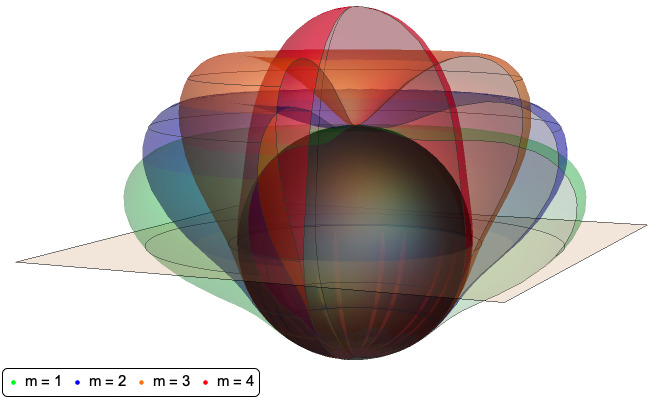
\includegraphics[width=9cm, height=5cm]{haldane eigenfunctions.jpg}
    \caption{\textit{Γραφική αναπαράσταση των ιδιοσυναρτήσεων για $s\subscr{0}=4$. Παρουσιάζονται τέσσερις από τις $2s\subscr{ο}+1$ ιδιοκαταστάσεις του τελεστή $L\subscr{z}$ με ιδιοτιμές $m\hbar$. (Πράσινο) $u\superscr{5}v\superscr{3}$ με $m=1$. (Μπλε) $u\superscr{6}v\superscr{2}$ με $m=2$. (Πορτοκαλί) $u\superscr{7}v$ με $m=3$. (Κόκκινο) $u\superscr{8}$ με $m=4$.}}
    \label{fig:haldane eigenfunctions s=4}
\end{figure}


%Για την περιγραφή σωματιδίου πάνω στη σφαίρα 
Προχωρούμε τώρα στη γραφική αναπαράσταση των πολυωνύμων Haldane \eqref{Haldane polynomial}. Καθορίζουμε αρχικά τις συνιστώσες $(a,b)$ του σπίνορα $\left| r\right>$ και τις εισάγουμε στην \eqref{Haldane polynomial}. 
%Οι συνιστώσες του $\left|r\right>$ είναι οι μιγαδικοί %συντελεστές των $2s\subscr{o}+1$ όρων στα πολυώνυμα Haldane και %προσδιορίζουν, όπως αναφέρθηκε προηγουμένως, το σημείο μέγιστης %πυκνότητας πιθανότητας. 
Για παράδειγμα, ας θεωρήσουμε τηω περίπτωση $s\subscr{0}=1$ και $\left|r\right>=(\cos\frac{\pi}{6}e\superscr{i\frac{\pi}{6}},\sin\frac{\pi}{6}e\superscr{-i\frac{\pi}{6}})$. Εφαρμόζοντας την \eqref{haldane wavefunction binomial}, η κυματοσυνάρτηση είναι
\begin{equation}
    \Psi\superscr{1}\subscr{r}\,=\,\sum\limits_{m=-1}^{1}\binom{2}{1+m}\left( \cos\frac{\pi}{6}\cos\frac{\theta}{2}e\superscr{i(\frac{\phi}{2}-\frac{\pi}{6})} \right)\superscr{1+m}\left( \sin\frac{\pi}{6}\sin\frac{\theta}{2} e\superscr{-i(\frac{\phi}{2}-\frac{\pi}{6})} \right)\superscr{1-m}
\end{equation}
Η αντίστοιχη πυκνότητα πιθανότητας φαίνεται στην εικόνα \ref{fig:haldane wavefunction s=1}. Είναι εμφανής η απουσία αζιμουθιακής συμμετρίας. Στη δεξιά εικόνα της \ref{fig:haldane wavefunction s=1}, απεικονίζεται μια τομή της γραφικής παράστασης, ώστε να διακρίνονται τα ακρότατα σημεία. Τα σημεία αυτά βρίσκονται αντιδιαμετρικά του $\vec{\Omega}\subscr{r}$. 
%, το διάνυσμα που συνδέεται με τον $\left|r\right>$ μέσω της %\eqref{position vector and spinor}. 
Στο σχήμα περιλαμβάνεται επίσης η μοναδιαία σφαίρα με κέντρο την αρχή των αξόνων.

\section{Πολυσωματιδιακές καταστάσεις φερμιονίων}
 Εάν αμελήσουμε τις αλληλεπιδράσεις μεταξύ των φορτισμένων σωματιδίων στις στάθμες Landau, η χαμιλτονιανή 
% αγνοώντας τις αλληλεπιδράσεις μεταξύ των φορτίων (integer hall %effect) 
 δίνεται από την έκφραση
\begin{equation*}
    H\,\approx\,\sum\subscr{i=1}\superscr{N}H\subscr{i}
\end{equation*}
όπου
\begin{figure}[t] 
    \centering
    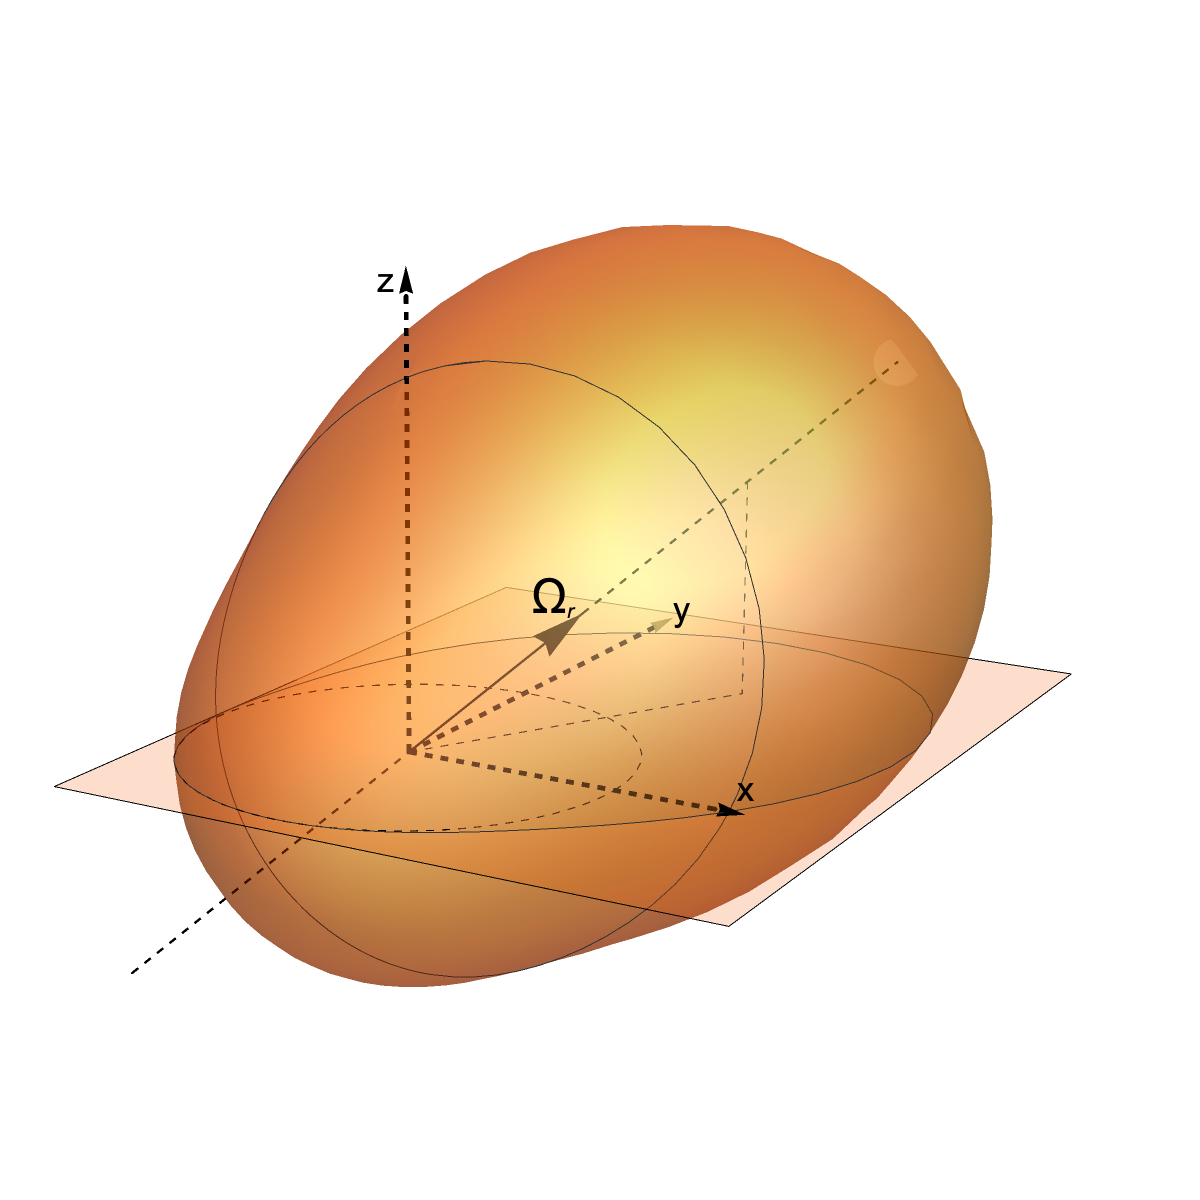
\includegraphics[width=7cm, height=8cm]{haldane wavefunction full.png}
    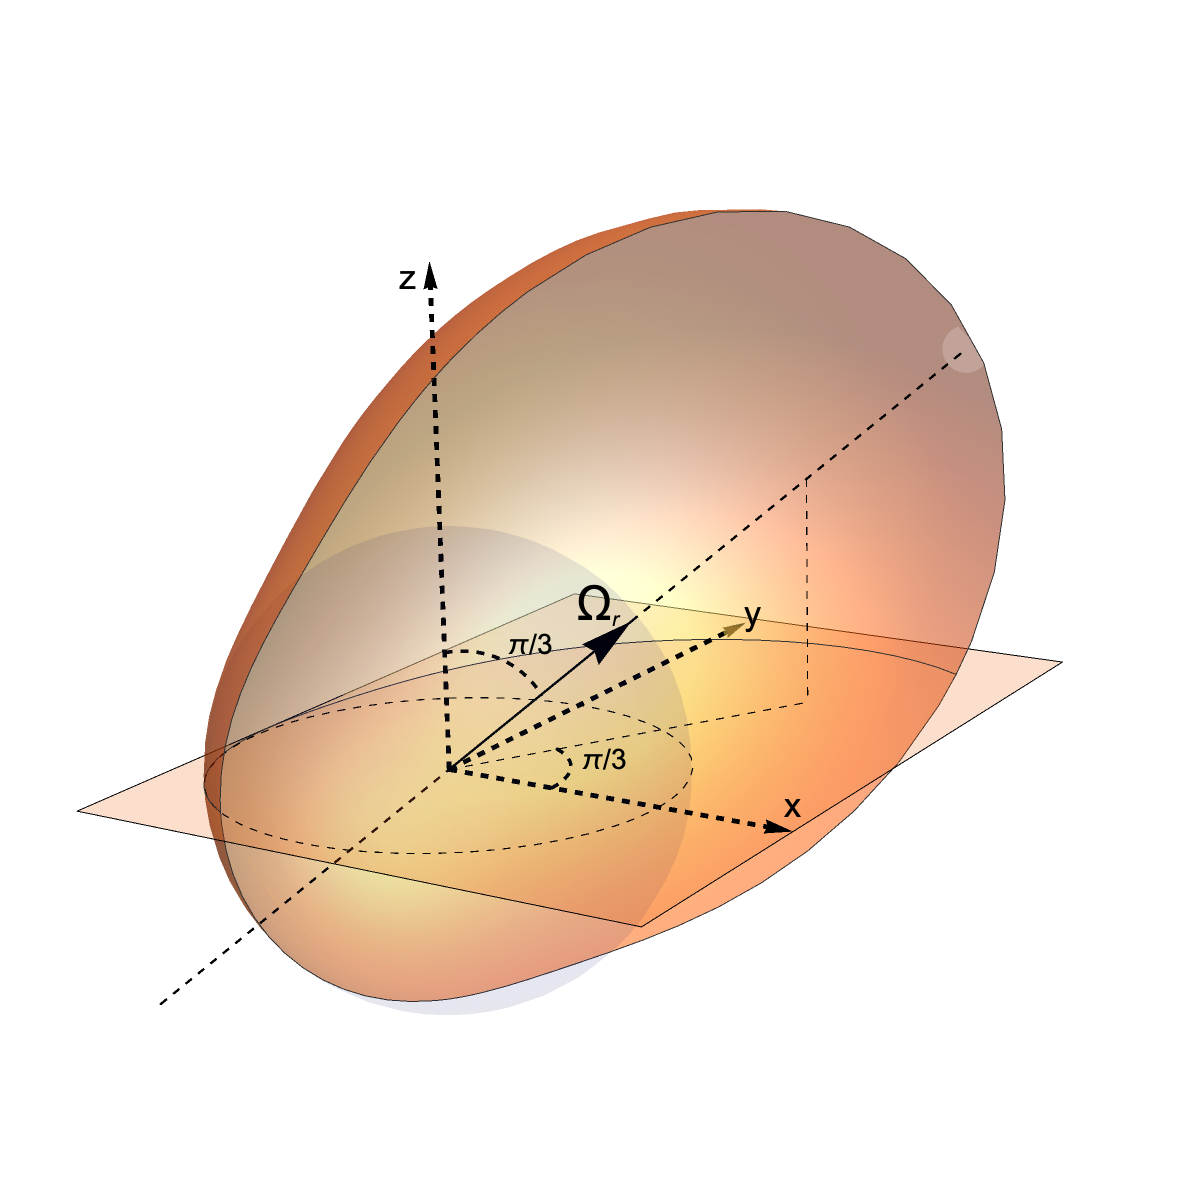
\includegraphics[width=7cm, height=8cm]{haldane wavefunction half.png}
    \caption{\textit{Γραφική αναπαράσταση της πυκνότητας πιθανότητας $|\Psi\superscr{1}\subscr{(a,b)}|^2$ για $s\subscr{0}=1$ και $\left|r\right>=(\cos\frac{\pi}{6}e\superscr{i\frac{\pi}{6}},\sin\frac{\pi}{6}e\superscr{-i\frac{\pi}{6}})$. Στο δεξιό σχήμα φαίνεται μια τομή της κυματοσυνάρτησης με το επίπεδο $\phi=\pi/3$, με μέγιστο στη θέση $\theta=\frac{\pi}{3},\phi=\frac{\pi}{3}$.}}
    \label{fig:haldane wavefunction s=1}
\end{figure}

%Η χαμιλτονιανή του συστήματος των Ν ασύζευτων σωματιδίων είναι %απλά το άθροισμα των μονοσωματιδιακών χαμιλτονιανών της μορφής \eqref{hamiltonian with magnetic monopole} 
\begin{equation*}
    H\subscr{i}\,=\,\frac{|\Lambda\subscr{i}|^2}{2m}\frac{eB}{\hbar s\subscr{0}}
\end{equation*}
η μονοσωματιδιακή χαμιλτονιανή.
%Η μηχανική στροφορμή $\Lambda\subscr{i}$ του σωματιδίου i %αντιστοιχεί στους γεννήτορες της άλγεβρας των περιστροφών %$L\subscr{i}$ 
(Ο δείκτης $i$ δηλώνει τα διάφορα σωματίδια).
%, όχι τις συνιστώσες) που ορίζονται όπως και στην \eqref{angular momentum algebra generators} και ικανοποιούν τις μεταθετικές σχέσεις \eqref{generator commutation relations}, ενώ μεταξύ δύο σωματιδίων i και j ισχύει ότι $[L\subscr{i},L\subscr{j}]=0$. 
Οι διάφορες μονοσωματιδιακές καταστάσεις καταλαμβάνονται σύμφωνα με την απαγορευτική αρχή του Pauli. Η ολική κυματοσυνάρτηση πρέπει να είναι αντισυμμετρική ως προς την εναλλαγή δύο οποιωνδήποτε φερμιονίων.
%Δεδομένου των προαναφερόμενων, είναι δυνατόν να φτιαχτεί %κατάσταση N σωματιδίων από το γινόμενο μονοσωματιδιακών %καταστάσεων. 
Όταν $N=2s\subscr{0}+1$, η χαμηλότερη στάθμη Landau είναι πλήρως κατειλημμένη. 
%LLL, αυτή δηλαδή των $N=2s\subscr{o}+1$ φερμιονίων, πρέπει να %γίνει η κατάληψη του LLL με τρόπο που σέβεται την απαγορευτική %αρχή του Pauli. Εφόσων έχουμε τόσα φερμιόνια όσος και ο %εκφυλισμός του LLL, 
Το κάθε φερμιόνιο καταλαμβάνει μια ανεξάρητη ορθογώνια μονοσωματιδιακή κατάσταση στη LLL, δες \eqref{basis of squared integrable functions on the sphere}.  
%ορθογώνια αυτής κάθε άλλου φερμιονίου. 
%Χρησιμοποιούμε τις ορθογώνιες μονοσωματιδιακές καταστάσεις %$\psi\subscr{s\subscr{o},m}$ της βάσης , με καλά ορισμένο κβαντικό %αριθμό m της z συνιστώσας της στροφορμής, $L\subscr{i,z}$. 
Προσδιορίζουμε την ολική κυματοσυνάρτηση $\Psi\subscr{N}$ 
%φτιάχνεται συνδυάζοντας τις $\psi\subscr{s\subscr{o},m}$ 
με χρήση της ορίζουσας Slater
\begin{equation}\label{slater determinant}
\Psi\subscr{N}\,=\,\left|\begin{array}{cccc}
    u\subscr{1}\superscr{2s\subscr{0}} & u\subscr{1}\superscr{2s\subscr{0}-1}v\subscr{1} &\dots & v\subscr{1}\superscr{2s\subscr{0}} \\
    u\subscr{2}\superscr{2s\subscr{0}} & \dots & \dots & v\subscr{2}\superscr{2s\subscr{0}} \\
    \vdots & \ddots & & \vdots\\
    u\subscr{N}\superscr{2s\subscr{0}} & u\subscr{N}\superscr{2s\subscr{0}-1}v\subscr{N} &\dots & v\subscr{N}\superscr{2s\subscr{0}}
\end{array}\right|
\end{equation}
%με τις σειρές του πίνακα να αντιστοιχούν σε ένα από τα %$2s\subscr{o}+1$ σωματίδια καθώς οι στήλες στις ιδιοκαταστάσεις %$\Psi\subscr{N}$. 
Η κυματοσυνάρτηση \eqref{slater determinant} γράφεται και στην ακόλουθη πιο απλή μορφή \cite{PhysRevLett.51.605}
\begin{equation}\label{haldane manyparticle wavefunction}
    \Psi\subscr{N}\,=\,\prod^{N}_{i<j}(u\subscr{i}v\subscr{j}-u\subscr{j}v\subscr{i})
\end{equation}
όπου $Ν$ ο εκφυλισμός της βασικής LLL (ή ο αριθμός των φερμιονίων)
\begin{equation}
    N=2s\subscr{0}+1
\end{equation}
Για συνοχή με τα προηγούμενα κεφάλαια 
%\cite{Maldacena_2021}, 
στα οποία η συνολική μαγνητική ροή συμβολίζεται με $Q$, θέτουμε $Q=2s_0$. Για μεγάλα $Q$, παίρνουμε λοιπόν
\begin{equation}
    N\approx Q\equiv 2s\subscr{0}
\end{equation}

\section{Εξίσωση διασποράς σχετικιστικών σωματιδίων}
%Στην περίπτωση κατάληψης του LLL από 
Για σχετικιστικά φερμιόνια με σπιν 1/2 και φορτίο $-e$, προσδιορίζουμε την εξίσωση διασποράς με βάση την εξίσωση Dirac. Σε επίπεδο χωροχρόνο, αυτή έχει τη μορφή
\begin{equation}\label{equation Dirac}
    \left( i \gamma\superscr{\mu}D\subscr{\mu} - m\right)\psi = 0
\end{equation}
όπου $\psi$ ο σπίνορας Dirac, $D\subscr{\mu}$ η συναλλοίωτη παράγωγος
\begin{equation}\label{covariant der}
\begin{split}
    &D\subscr{\mu}\equiv\partial\subscr{\mu}-ieA\subscr{\mu}\\
    &[D\subscr{\mu},D\subscr{\nu}]=-ieF\subscr{\mu\nu}
\end{split}
\end{equation}
και $F\subscr{\mu\nu}$ ο ηλεκτρομαγνητικός τανυστής του Maxwell
\begin{equation}
    F\subscr{\mu\nu}=\partial\subscr{\mu}A\subscr{\nu}-\partial\subscr{\nu}A\subscr{\mu}
\end{equation}
Δρούμε στα δύο μέλη της \eqref{equation Dirac} με τον μιγαδικό συζυγή του τελεστή Dirac και καταλήγουμε στην εξίσωση
\begin{equation}\label{dirac equation to klein gordon}
    (\gamma\superscr{\mu}\gamma\superscr{\nu}D\subscr{\mu}D\subscr{\nu}+m\superscr{2})\psi\,=\,0
\end{equation}
Με χρήση του μεταθέτη \eqref{gamma matrix commutator} και του αντιμεταθέτη \eqref{gamma matrix anticommutator} των πινάκων Dirac, η \eqref{dirac equation to klein gordon} παίρνει τη μορφή
\begin{equation}
    \frac{1}{2}(-4iS\superscr{\mu\nu}D\subscr{\mu}D\subscr{\nu}+2D\superscr{\mu}D\subscr{\mu})\psi+m\superscr{2}\psi\,=\,0
\end{equation}
Ο μεταθέτης \eqref{covariant der} εισάγει στην εξίσωση τον ηλεκτρομαγνητικό τανυστή
\begin{equation}
    \left[D\superscr{2} - iS\superscr{\mu\nu}(-ieF\subscr{\mu\nu}) +m\superscr{2}\right]\psi\,=\,0
\end{equation}
%της μορφής του $F\subscr{\mu\nu}$ 
Στην περίπτωση μη μηδενικού μαγνητικού πεδίου (δες \eqref{def of em tensor}) 
\begin{equation}
    \begin{split}
        &F\subscr{0i}=F\subscr{i0}=0\\
        &F\subscr{ij}=\epsilon\subscr{ijk}B\subscr{k}
    \end{split}
\end{equation}
όπου $B_k$ οι συνιστώσες του μαγνητικού πεδίου, και χρσιμοποιώντας την εκφραση του $S\superscr{\mu\nu}$ \cite{Peskin:1995ev}, η σχετικιστική εξίσωση ανάγεται στην
\begin{equation}\label{relativistic energy equation}
    \left[ D\superscr{2}\subscr{0}+(-iD\subscr{i})\superscr{2}-2e\Vec{B}\cdot\Vec{S}+m\superscr{2} \right]\psi\,=\,0
\end{equation}
Μετασχηματίζοντας στο χώρο των ορμών, ο πρώτος όρος δείνει το αρνητικό τετράγωνο της ενέργειας $-E\superscr{2}$ 
%όταν δράσει στην $\psi$ 
ενώ ο δεύτερος περιλαμβάνει τον τελεστή της μηχανικής ορμής, ο οποίος συνδέεται με την στροφορμή \eqref{mechanical momentum} ως εξής
\begin{equation}
    \Vec{\Pi}\superscr{2}\,=\,\frac{1}{r\superscr{2}}\left[ \Vec{\Lambda}\superscr{2}-i\Vec{r}\cdot\Vec{\Pi}+(\Vec{r}\cdot\Vec{\Pi})\superscr{2} \right]\,=\,\frac{\Lambda\superscr{2}}{r\superscr{2}}-\frac{1}{r\superscr{2}}\frac{\partial}{\partial r}r\superscr{2}\frac{\partial}{\partial r}
\end{equation}
Συμβολίζουμε την ακτινική ορμή με $p\subscr{3}$ 
\begin{equation}
     \Vec{\Pi}\superscr{2}\,=\,\frac{\Lambda\superscr{2}}{r\superscr{2}}+p\subscr{3}\superscr{2}
\end{equation}
Αντικαθιστούμε την ιδιοτιμή του τελεστή $\Lambda\superscr{2}$, δες \eqref{eigenvalues in LLL}, και βρίσκουμε 
\begin{equation}
    \frac{\Lambda\superscr{2}}{r\superscr{2}}=\frac{s\subscr{0}}{r\superscr{2}}=eB\equiv |F|
\end{equation}
Ο τρίτος όρος περιγράφει την αλληλεπίδραση του μαγνητικού πεδίου με το σπιν $\Vec{S}$
\begin{equation}
    2e\Vec{B}\cdot\Vec{S} = 2eBs \equiv 2|F|s
\end{equation}
%Στην $\ell$ αναπαράσταση της ομάδας Lorentz ο τελεστής S έχει %ιδιοτιμές $s=-\ell,\dots,\ell-1,\ell$. Συγκεκριμένα, για την %$\frac{1}{2}$ αναπαράσταση 
Για ένα φερμιόνιο οι ιδιοτιμές του σπιν είναι $\pm\frac{1}{2}$ (θέτουμε $\hbar=1$ ) από τις οποίες επιλέγεται η θετική για ισχυρά μαγνητικά πεδία. Ως αποτέλεσμα, να αλληλοαναιρούνται η ενεργειακή συνεισφορά εξαιτίας της αλληλεπίδρασης της τροχιακής στροφορμής με το μαγνητικό πεδίο και η συνεισφορά εξαιτίας της σύζευξης του σπιν με το μαγνητικό πεδίο. 
Τέλος, με βάση τα πιο πάν, η σχετικιστική εξίσωση διασποράς ανάγεται στην ακόλουθη
\begin{equation}\label{spinor energy magnetic field}
    E\superscr{2}(\text{spinor})-p\subscr{3}\superscr{2}\,=\,m\superscr{2}+|F|(1-2s)=m\superscr{2}+0,\qquad s=1/2
\end{equation}
\\

Για βαθμωτά πεδία (με σπιν $0$) και φορτίο $-e$, η αντίστοιχη εξίσωση είναι 
%ενέργεια δεν περιέχει τη σύζευξη μεταξύ spin και μαγνητικού %πεδίου και είναι
\begin{equation}\label{scalar energy}
     E\superscr{2}(\text{scalar})-p\subscr{3}\superscr{2}\,=\,m\superscr{2}+|F|,\qquad s=0
\end{equation}
Για φορτισμένα διανυσματικά πεδία με σπιν $1$ παίρνουμε \cite{Corben:1940zz}
%αναπαράστασης ισχύει η εξίσωση \eqref{spinor energy magnetic %field} της σπινορικής αναπαράστασης. Ο γυρομαγνητικός λόγος %$\gamma=2$ των σπιν 1 πεδίων φέρει τις ενεργειακές ιδιότητες %της αναπαράστασης, εντός μαγνητικού πεδίου, πολύ κοντά σε αυτές %των σπινόρων Dirac. Η σύζευξη των σπιν 1 πεδίων με %ηλεκτρομαγνητικό πεδίο και ο γυρομαγνητικός λόγος %παρουσιάζονται στο άρθρο  των Corben και Schwinger. H ενέργεια %για την ιδιοτιμή $s=1$ είναι 
\begin{equation}\label{vector boson energy magnetic field}
    E\superscr{2}(\text{vector})-p\subscr{3}\superscr{2}\,=\,m\superscr{2}+|F|(1-2s)=m\superscr{2}-|F|,\qquad s=1
\end{equation}
\\
%%%%%%%%%%%%%%%%%%%%%%%%%%%%%%%%%%%%%%%%%%%%%%%%%%%%%%%%%%%%%%%%%%%%%%%%%%%%%
%%%%%%%%%%%%%%%%%%%%%%%%%%%%%%%%%%%%%%%%%%%%%%%%%%%%%%%%%%%%%%%%%%%%%%%%%%%%%
Συνοψίζοντας τα παραπάνω, στη βασική στάθμη Landau $n=0$, οι εξισώσεις διασποράς για φορτισμένα βαθμωτά, φερμιονικά και διανυσματικά  πεδία είναι
\begin{equation}
    E\superscr{2}-p\subscr{3}\superscr{2}\,=\,\left\{\begin{array}{ll}
         m\superscr{2}+|F|, &s=0 \\
         m\superscr{2}+0, & s=1/2 \\
         m\superscr{2}-|F|, & s=1
    \end{array}\right.
\end{equation}

%%%%%%%%%%%%%%%%%%%%%%%%%%%%%%%%%%%%%%%%%%%%%%%%%%%%%%%%%%%%%%%%%%%%%%%%%%%%%
%%%%%%%%%%%%%%%%%%%%%%%%%%%%%%%%%%%%%%%%%%%%%%%%%%%%%%%%%%%%%%%%%%%%%%%%%%%%%
\begin{comment}
\section{Προχειρο}
και έτσι αναθέτουμε σε κάθε σωματίδιο μια ιδιοκατάσταση του 
Όταν το εκφυλισμένο χαμηλότερο επίπεδο Landau είναι πλήρως κατηλημένο από φερμιόνια η συνολική στροφορμή μηδενίζεται, $\Vec{L}=\sum_{i}^{\text{\scalebox{0.6}{$2s\subscr{o}+1$}}}\Vec{L\subscr{i}}=0$ - κάθε μία από τις $2s\subscr{o}+1$ ιδιοκαταστάσεις καταλαμβάνεται από ένα μόνο φερμιόνιο. Επομένως, δεν χρειάζεται να οριστεί διάνυσμα $\Omega\subscr{r}\text{\scalebox{0.7}{$(a,b)$}}$, όπως υπάρχει για παράδειγμα στην μονοσωματιδιακή κυματοσυνάρτηση \eqref{Haldane polynomial}, και έτσι η $\Psi\subscr{N}$ είναι ανεξάρτητη των (a,b). Σύμφωνα με την απαγορευτική αρχή του Pauli η $\Psi\subscr{N}$ πρέπει να είναι πλήρως αντισυμμετρική ως προς εναλλαγή δύο οποιωνδήποτε σωματιδίων. \\

Στο κείμενο του, ο Haldane, παρουσιάζει μεταξύ άλλων την αντισυμμετρική κυματοσυνάρτηση δύο φερμιονίων $\psi_{\text{\scalebox{0.8}{(a,b)}}}^{\text{\scalebox{0.8}{($s\subscr{o}$,j)}}}$. Στην παρουσία δύο σωματιδίων ο τελεστής της συνολικής στροφορμής είναι $\Vec{L}=\Vec{L}\subscr{1}+\Vec{L}\subscr{2}$. Ο τελεστής $L\superscr{2}$ έχει ιδιοτιμές j(j+1) όπου j παίρνει κβαντωμένες τιμές από 0 ($L\subscr{1}$, $L\subscr{2}$ αντιπαράλληλα) μέχρι 2$s\subscr{o}$ ($L\subscr{1}$, $L\subscr{2}$ παράλληλα) - στο LLL. Περιγράφει τις καταστάσεις με τα πολυώνυμα που ικανοποιούν την εξίσωση ιδιοτιμών
\begin{equation}
    \{\Omega\subscr{r}\cdot\Vec{L}\} \psi_{\text{\scalebox{0.8}{(a,b)}}}^{\text{\scalebox{0.8}{($s\subscr{o}$,j)}}}\,=\,\hbar j\,\psi_{\text{\scalebox{0.8}{(a,b)}}}^{\text{\scalebox{0.8}{($s\subscr{o}$,j)}}} \qquad 0\le\,j\,\le\,2s\subscr{o}
\end{equation}
Όπως και στην μονοσωματιδιακή περίπτωση έτσι και τώρα, η $\psi_{\text{\scalebox{0.8}{(a,b)}}}^{\text{\scalebox{0.8}{($s\subscr{o}$,j)}}}$ επικεντρώνεται γύρω από το σημείο με διάνυσμα $\Omega\subscr{r}(a,b)$ αντίστοιχο του σπίνορα (a,b)
\begin{equation}
    \psi_{\text{\scalebox{0.8}{(a,b)}}}^{\text{\scalebox{0.8}{($s\subscr{o}$,j)}}} \,=\, (u\subscr{1}v\subscr{2}-u\subscr{2}v\subscr{1})\superscr{2s\subscr{o}-j}\prod\limits_{i=1,2}(a\superscr{*}u\subscr{i}+b\superscr{*}v\subscr{i})\superscr{j}
\end{equation}
\end{comment}
